% Created by tikzDevice version 0.12.6 on 2026-08-08 02:44:58
% !TEX encoding = UTF-8 Unicode
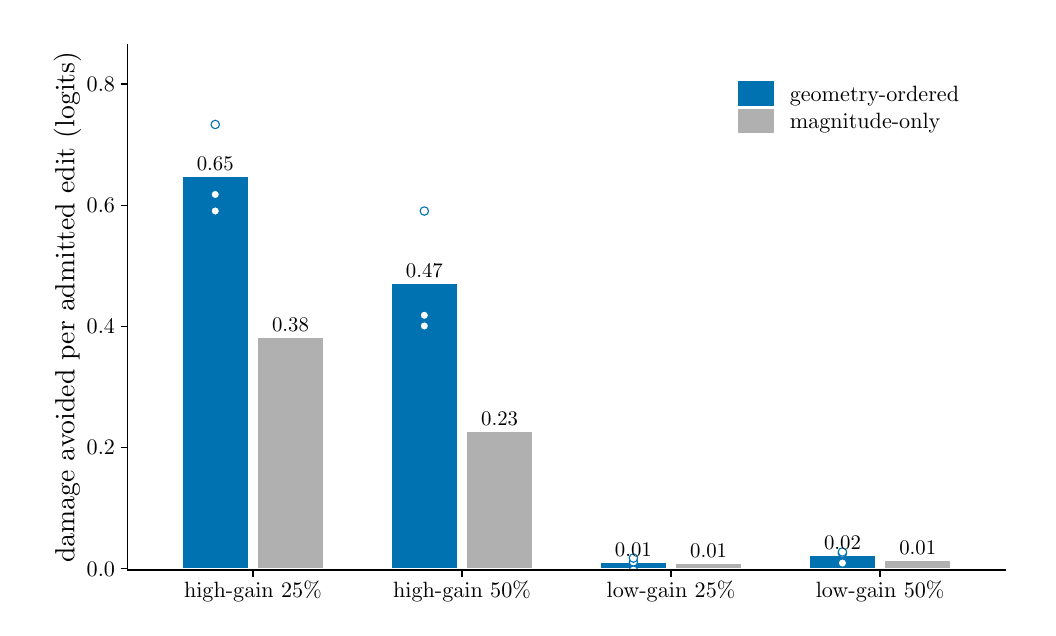
\begin{tikzpicture}[x=1pt,y=1pt]
\definecolor{fillColor}{RGB}{255,255,255}
\path[use as bounding box,fill=fillColor,fill opacity=0.00] (0,0) rectangle (361.35,209.58);
\begin{scope}
\path[clip] (  0.00,  0.00) rectangle (361.35,209.58);
\definecolor{drawColor}{RGB}{255,255,255}
\definecolor{fillColor}{RGB}{255,255,255}

\path[draw=drawColor,line width= 0.5pt,line join=round,line cap=round,fill=fillColor] ( -0.00,  0.00) rectangle (361.35,209.58);
\end{scope}
\begin{scope}
\path[clip] ( 36.05, 13.56) rectangle (353.35,203.58);
\definecolor{fillColor}{RGB}{255,255,255}

\path[fill=fillColor] ( 36.05, 13.56) rectangle (353.35,203.58);
\definecolor{fillColor}{RGB}{0,114,178}

\path[fill=fillColor] ( 56.07, 14.18) rectangle ( 79.49,155.74);
\definecolor{fillColor}{gray}{0.69}

\path[fill=fillColor] ( 83.27, 14.18) rectangle (106.69, 97.45);
\definecolor{fillColor}{RGB}{0,114,178}

\path[fill=fillColor] (131.62, 14.18) rectangle (155.04,116.94);
\definecolor{fillColor}{gray}{0.69}

\path[fill=fillColor] (158.82, 14.18) rectangle (182.24, 63.55);
\definecolor{fillColor}{RGB}{0,114,178}

\path[fill=fillColor] (207.17, 14.18) rectangle (230.59, 16.01);
\definecolor{fillColor}{gray}{0.69}

\path[fill=fillColor] (234.36, 14.18) rectangle (257.78, 15.91);
\definecolor{fillColor}{RGB}{0,114,178}

\path[fill=fillColor] (282.71, 14.18) rectangle (306.13, 18.64);
\definecolor{fillColor}{gray}{0.69}

\path[fill=fillColor] (309.91, 14.18) rectangle (333.33, 16.71);
\definecolor{drawColor}{RGB}{0,114,178}
\definecolor{fillColor}{RGB}{255,255,255}

\path[draw=drawColor,line width= 0.4pt,line join=round,line cap=round,fill=fillColor] ( 67.78,174.60) circle (  1.53);

\path[draw=drawColor,line width= 0.4pt,line join=round,line cap=round,fill=fillColor] ( 67.78,149.31) circle (  1.53);

\path[draw=drawColor,line width= 0.4pt,line join=round,line cap=round,fill=fillColor] ( 67.78,143.34) circle (  1.53);

\path[draw=drawColor,line width= 0.4pt,line join=round,line cap=round,fill=fillColor] (143.33,143.32) circle (  1.53);

\path[draw=drawColor,line width= 0.4pt,line join=round,line cap=round,fill=fillColor] (143.33,105.65) circle (  1.53);

\path[draw=drawColor,line width= 0.4pt,line join=round,line cap=round,fill=fillColor] (143.33,101.80) circle (  1.53);

\path[draw=drawColor,line width= 0.4pt,line join=round,line cap=round,fill=fillColor] (218.88, 16.52) circle (  1.53);

\path[draw=drawColor,line width= 0.4pt,line join=round,line cap=round,fill=fillColor] (218.88, 17.92) circle (  1.53);

\path[draw=drawColor,line width= 0.4pt,line join=round,line cap=round,fill=fillColor] (218.88, 13.56) circle (  1.53);

\path[draw=drawColor,line width= 0.4pt,line join=round,line cap=round,fill=fillColor] (294.42, 19.65) circle (  1.53);

\path[draw=drawColor,line width= 0.4pt,line join=round,line cap=round,fill=fillColor] (294.42, 20.13) circle (  1.53);

\path[draw=drawColor,line width= 0.4pt,line join=round,line cap=round,fill=fillColor] (294.42, 16.12) circle (  1.53);
\definecolor{drawColor}{RGB}{0,0,0}

\node[text=drawColor,anchor=base,inner sep=0pt, outer sep=0pt, scale=  0.75] at ( 67.78,158.08) {0.65};

\node[text=drawColor,anchor=base,inner sep=0pt, outer sep=0pt, scale=  0.75] at ( 94.98, 99.79) {0.38};

\node[text=drawColor,anchor=base,inner sep=0pt, outer sep=0pt, scale=  0.75] at (143.33,119.28) {0.47};

\node[text=drawColor,anchor=base,inner sep=0pt, outer sep=0pt, scale=  0.75] at (170.53, 65.88) {0.23};

\node[text=drawColor,anchor=base,inner sep=0pt, outer sep=0pt, scale=  0.75] at (218.88, 18.35) {0.01};

\node[text=drawColor,anchor=base,inner sep=0pt, outer sep=0pt, scale=  0.75] at (246.07, 18.24) {0.01};

\node[text=drawColor,anchor=base,inner sep=0pt, outer sep=0pt, scale=  0.75] at (294.42, 20.98) {0.02};

\node[text=drawColor,anchor=base,inner sep=0pt, outer sep=0pt, scale=  0.75] at (321.62, 19.05) {0.01};
\end{scope}
\begin{scope}
\path[clip] (  0.00,  0.00) rectangle (361.35,209.58);
\definecolor{drawColor}{RGB}{0,0,0}

\path[draw=drawColor,line width= 0.5pt,line join=round,line cap=rect] ( 36.05, 13.56) --
	( 36.05,203.58);
\end{scope}
\begin{scope}
\path[clip] (  0.00,  0.00) rectangle (361.35,209.58);
\definecolor{drawColor}{RGB}{0,0,0}

\node[text=drawColor,anchor=base east,inner sep=0pt, outer sep=0pt, scale=  0.80] at ( 31.55, 11.42) {0.0};

\node[text=drawColor,anchor=base east,inner sep=0pt, outer sep=0pt, scale=  0.80] at ( 31.55, 55.17) {0.2};

\node[text=drawColor,anchor=base east,inner sep=0pt, outer sep=0pt, scale=  0.80] at ( 31.55, 98.92) {0.4};

\node[text=drawColor,anchor=base east,inner sep=0pt, outer sep=0pt, scale=  0.80] at ( 31.55,142.66) {0.6};

\node[text=drawColor,anchor=base east,inner sep=0pt, outer sep=0pt, scale=  0.80] at ( 31.55,186.41) {0.8};
\end{scope}
\begin{scope}
\path[clip] (  0.00,  0.00) rectangle (361.35,209.58);
\definecolor{drawColor}{RGB}{0,0,0}

\path[draw=drawColor,line width= 0.5pt,line join=round] ( 33.55, 14.18) --
	( 36.05, 14.18);

\path[draw=drawColor,line width= 0.5pt,line join=round] ( 33.55, 57.92) --
	( 36.05, 57.92);

\path[draw=drawColor,line width= 0.5pt,line join=round] ( 33.55,101.67) --
	( 36.05,101.67);

\path[draw=drawColor,line width= 0.5pt,line join=round] ( 33.55,145.42) --
	( 36.05,145.42);

\path[draw=drawColor,line width= 0.5pt,line join=round] ( 33.55,189.16) --
	( 36.05,189.16);
\end{scope}
\begin{scope}
\path[clip] (  0.00,  0.00) rectangle (361.35,209.58);
\definecolor{drawColor}{RGB}{0,0,0}

\path[draw=drawColor,line width= 0.5pt,line join=round,line cap=rect] ( 36.05, 13.56) --
	(353.35, 13.56);
\end{scope}
\begin{scope}
\path[clip] (  0.00,  0.00) rectangle (361.35,209.58);
\definecolor{drawColor}{RGB}{0,0,0}

\path[draw=drawColor,line width= 0.5pt,line join=round] ( 81.38, 11.06) --
	( 81.38, 13.56);

\path[draw=drawColor,line width= 0.5pt,line join=round] (156.93, 11.06) --
	(156.93, 13.56);

\path[draw=drawColor,line width= 0.5pt,line join=round] (232.47, 11.06) --
	(232.47, 13.56);

\path[draw=drawColor,line width= 0.5pt,line join=round] (308.02, 11.06) --
	(308.02, 13.56);
\end{scope}
\begin{scope}
\path[clip] (  0.00,  0.00) rectangle (361.35,209.58);
\definecolor{drawColor}{RGB}{0,0,0}

\node[text=drawColor,anchor=base,inner sep=0pt, outer sep=0pt, scale=  0.80] at ( 81.38,  3.56) {high-gain 25\%};

\node[text=drawColor,anchor=base,inner sep=0pt, outer sep=0pt, scale=  0.80] at (156.93,  3.56) {high-gain 50\%};

\node[text=drawColor,anchor=base,inner sep=0pt, outer sep=0pt, scale=  0.80] at (232.47,  3.56) {low-gain 25\%};

\node[text=drawColor,anchor=base,inner sep=0pt, outer sep=0pt, scale=  0.80] at (308.02,  3.56) {low-gain 50\%};
\end{scope}
\begin{scope}
\path[clip] (  0.00,  0.00) rectangle (361.35,209.58);
\definecolor{drawColor}{RGB}{0,0,0}

\node[text=drawColor,rotate= 90.00,anchor=base,inner sep=0pt, outer sep=0pt, scale=  1.00] at ( 16.89,108.57) {damage avoided per admitted edit (logits)};
\end{scope}
\begin{scope}
\path[clip] (  0.00,  0.00) rectangle (361.35,209.58);
\definecolor{fillColor}{RGB}{255,255,255}

\path[fill=fillColor] (255.93,180.78) rectangle (270.38,190.78);
\definecolor{fillColor}{RGB}{0,114,178}

\path[fill=fillColor] (256.57,181.43) rectangle (269.73,190.13);
\end{scope}
\begin{scope}
\path[clip] (  0.00,  0.00) rectangle (361.35,209.58);
\definecolor{fillColor}{RGB}{255,255,255}

\path[fill=fillColor] (255.93,170.78) rectangle (270.38,180.78);
\definecolor{fillColor}{gray}{0.69}

\path[fill=fillColor] (256.57,171.43) rectangle (269.73,180.13);
\end{scope}
\begin{scope}
\path[clip] (  0.00,  0.00) rectangle (361.35,209.58);
\definecolor{drawColor}{RGB}{0,0,0}

\node[text=drawColor,anchor=base west,inner sep=0pt, outer sep=0pt, scale=  0.80] at (275.38,183.03) {geometry-ordered};
\end{scope}
\begin{scope}
\path[clip] (  0.00,  0.00) rectangle (361.35,209.58);
\definecolor{drawColor}{RGB}{0,0,0}

\node[text=drawColor,anchor=base west,inner sep=0pt, outer sep=0pt, scale=  0.80] at (275.38,173.03) {magnitude-only};
\end{scope}
\end{tikzpicture}
